\documentclass[]{article}
\usepackage{amsmath}
\usepackage{mathtools}
\usepackage{fullpage}
\usepackage{graphicx}
\usepackage{color}
\usepackage[a4paper]{geometry}

\begin{document}

\title{Response letter}
  \author{Luis Sanabria-Russo, Jaume Barcelo, Boris Bellalta, Francesco Gringoli}

\date{\today}
\maketitle
\emph{Authors sincerely appreciate the time spent reading our work. Your insight propelled new considerations and discoveries that contributed to futher improve the paper. Thank you. \\\\This latter presents our responses to all the reviewers's comments. Additionnally, it provides an overview of the new contributions included in the paper. Authors kindly suggest to read it through, as some answers built on previous explanations. Again, thank you very much.\\}

In this new version of the paper, the more relevant additions are:
\begin{itemize}
	\item Completely redrawn set of figures with clearer explanations.
	\item A throughput comparison with similar reservation-like collision-free MAC protocols for IEEE 802.11 networks.
	\item Analysis of the impact of channel errors over CSMA/ECA$_{\text{Hys+FS}}$'s deterministic backoff.
	\item A new mechanism for reducing the length of collision-free schedules in CSMA/ECA$_{\text{Hys+FS}}$.
	\item The first experimental results of a real hardware implementation of CSMA/ECA with Hysteresis.
\end{itemize}

\section*{Including a new author}
We replaced an entire section with the first real hardware implementation of CSMA/ECA with Hysteresis. To achieve such feat of low-level code customisation and testbed configuration we relied on the experience of professor Francesco Gringoli. It is our pleasure to include his contribution to the rest of the work and to add his name to the list of authors.

\section*{Number of pages}
Authors agree with the Reviewers's suggestions on extending the related work Section. Nevertheless, it was decided to pay especial attention clarifying key Reviewers's comments. In doing so, we slightly exceeded the page limit. Authors apologise for this inconvenience and kindly ask the Reviewers to take the value added to the whole contribution as consideration for its approval.

\section{Reviewer 1}
The authors appreciate your contribution in enhancing the readability of the work. We are pleased to show a more accessible text, with better punctuation; standardised set of Figures and thorough explanations. 


	\subsection{Regarding ``Abstract"}
		Changes from \emph{``totally distributed"} to fully decentralised were made throughout the document.
	
	\subsection{Regarding ``Introduction"}
		\begin{itemize}
			\item {\bfseries What would be useful in the Introduction to specifically mention, is whether the proposed CSMA solution performs well when co-existing [perhaps with more greedy?] legacy CSMA/CA clients. The authors mention that throughput improves in co-existance scenarios, but it should be clear that it is not at the cost of better throughput for the nodes that are operating using the authors' proposed CSMA solution. This leaves less room for reader drifts.}
		\end{itemize}
		
		\begin{figure}[tb]
		\centering
			\includegraphics[width=0.45\linewidth,angle=-90]{figures/saturated/mixed/throughput-per-protocol/throughput-per-protocol-TON.eps}
			\caption{Average station throughput per MAC protocol in a saturated mixed network}
			\label{fig:coex}
		\end{figure}
		
		We appreciate the observation. CSMA/CA nodes are in fact very greedy. Nevertheless, in an mixed scenario example where half the nodes run CSMA/CA and half CSMA/ECA$_{\text{Hys+FS}}$, we observe a throughput enhancement for CSMA/CA when compared against a CSMA/CA-only network. This is now referred in the document in the following way:\\
		
		`\emph{As tests in a mixed network with different proportions of CSMA/CA and CSMA/ECA nodes show, the aggregated throughput is higher than the observed in CSMA/CA-only networks. Furthermore, at low number of total contenders CSMA/CA's throughput is actually improved, while it is degraded in crowded scenarios. This constitutes a motivation for a change towards CSMA/ECA.}'\\
		
		This is further assessed at Section V regarding Figure~\ref{fig:coex} in this letter:\\
		
		`\emph{It is possible to see that for a low total number contenders ($N^{*}\leq 12$) CSMA/CA stations attain greater throughput than in a CSMA/CA-only network. Again, this is because in the mixed network setup the other $N^{*}/2$ contenders with CSMA/ECA$_{\text{Hys+FS}}$ use a deterministic backoff, leaving many empty slots between transmissions.}'
		
		`\emph{...for $N^{*}>12$ periods of collision-free operation and the aggregation performed with Fair Share allows CSMA/ECA$_{\text{Hys+FS}}$ to have larger channel time than CSMA/CA nodes, which throughput degrades even more than in CSMA/CA-only. These results suggests that a switch to CSMA/ECA$_{\text{Hys+FS}}$ can be beneficial for networks with high number of contenders.}'
		
		\begin{itemize}
			\item {\bfseries An implementation is crucial as well as the use of a measurement-based simulation environment. Good work. Mention in the introduction that the simulation is based on the COST simulation environment for greater credibility.}
		\end{itemize}
		
		We included a reference to a new customization of the COST simulator and incorporated a completely new hardware implementation Section.
		
	\subsection{Regarding ``Related Work"}
		\begin{itemize}
			\item {\bfseries When stating the size $N$ of  collision slots, and that solutions that adopt such policies do not take care of situations where the number of nodes $M > N$, please give an example value for $N$. What number of M are we looking at? And is it reasonable to make the argument that $M > N$? If $N$ is large as it is, then the concern is not that $M > N$, but really can we service that many nodes? (at least not [reasonably] today) Perhaps a simple footnote could help clarify this.}
		\end{itemize}
		
		IEEE 8011.ax Task Group suggest simulation scenarios with $10's$ to $100's$ of stations for a single Access Point (AP). Based on the current minimum Contention Window (CW$_{\min}=16$) we can safely take an example of number of slots in a schedule, $N$ to be $16$ or $8$ slots. That is, collision-free schedules can be built with no more than $M\leq N$ contenders. When $M>N$ collisions will reappear, contributing to the observed overall throughput degradation. 
		
		It is clear that a flexible or adjustable schedule is needed for collision-free operation with many contenders, as it is proposed in this work. Nevertheless, when $M$ is very big, say 200 contenders, and assuming $M\leq N$, the process of converging to a collision-free schedule will provoke some collisions, further degrading the overall throughput as the number of contenders increases. Besides, the increased time between successful transmissions will also degrade the average throughput of each node, but still keeping it higher than a CSMA/CA node.

	\subsection{Regarding ``Section III"}
		\begin{itemize}
			\item {\bf It would be useful if the authors include a table with a list of important notations. Would help with readability.}
		\end{itemize}

		We now include a short table (Table I in the paper) with useful notation regarding backoff procedure variables and different CSMA/ECA configurations.

		\begin{itemize}
			\item {\bfseries Section III.B, the aggregation process should be explained in more detail. Is the aggregation here similar to that used in 802.11n, where the level of aggregation depends on the transmission rate? How are packets aggregated? It is then mentioned in Section III.C that the packet is an MPDU and other details that indicate this protocol is applied for 802.11n+. Please clarify these details before then.}
		\end{itemize}
		
 		The authors apologise for raising any confusion. The aggregation performed with Fair Share does not depend on 		the rate. In fact, it only depends on the backoff stage at the moment of transmission. That is, stations at backoff 		stage $k$ will aggregate and transmit an A-MPDU frame with $2^{k}$ data frames. This is done with the sole 			purpose of providing fairness to CSMA/ECA$_{\text{Hys}}$ stations with different deterministic backoffs.
		
		We now first refer to Fair Share mentioning the following:\\
		
		`\emph{Fair Share is an A-MPDU aggregation mechanism that coupled with the collision-free schedule built by CSMA/ECA$_{\text{Hys}}$ is able to provide short-term fairness. However, it also improves the throughput since the aggregation process makes the packet transmission more efficient by reducing overheads. Furthermore, the level of aggregation provided by Fair Share depends on the buffer occupancy and the current backoff stage.}'
		
		\begin{itemize}
			\item {\bfseries It is not clear in Section III.C what the authors mean by the "inferior" backoff stage. Please clarify or replace with a more descriptive word. Perhaps: subsequent, later, following, etc.}
		\end{itemize}
		
		We extended the explanation everywhere this could cause confusion. Authors kindly refer the Reviewer to Section III-C in the paper.
		
	\subsection{Regarding ``Simulation"}
		\begin{itemize}
			\item {\bfseries The component lines in Figure 9 are not clear. They overlap. Perhaps in all graphs, align the legends with the order of their corresponding results. For example, the first legend item corresponds to the largest result (as in Figure 10). Also, this reader suggests to add a major line to separate the two parts of Figure 9 for more clarity --- this applies to other figures too. Also, more discussion on the values for the average backoff stage. What do large/small values mean? What kind of best pattern are we looking for? Results aren't as intuitive as other metrics.}
		\end{itemize}
		
		We completely regenerated the figures. All the legends follow the order of appearance of the curves in the Figure. We chose to group related figures together to save space and improve the structure of the paper.
		
		Backoff stages reflect the length of the collision-free schedule (if any) in CSMA/ECA$_{\text{Hys+FS}}$. When increasing the number of contenders in a network, it is expected to see an increase in the average backoff stage of each node given that a larger schedule length is needed to allocate those users (as can be observed in Figure 7a in the paper). Furthermore, in saturated scenarios with channel errors nodes will rapidly end up in the maximum backoff stage due to failed transmissions, and therefore use the largest deterministic backoff.
			
		On the other hand, in non-saturated traffic conditions we see an increase of the average backoff stage when the network approaches the saturation point (see Figure 8a in the paper). This is because CSMA/ECA and CSMA/CA reset their backoff stage to zero when the MAC queue empties.
		
		The ideal solution is to reach collision-free operation with the lowest backoff stage possible. This may affect the aggregation performed by Fair Share, but at the same decreases the time between successful transmissions and increases the channel utilization.
		
		\begin{itemize}
			\item {\bf A little more detail on the peak values at around 35 nodes for the proposed solution. In Figure 15 and 16, it appears as if 35 nodes would be the worst-case scenario for a network to remain in. Some explanation on how the dropped packets (or collision slot) increase is a temporary result before the network re-calibrates and that values in the long-run look more like the values for other N values.}
		\end{itemize}
		
		We provided an extended explanation for this case. Basically, when $20 < N \leq 35$ there are not enough transmissions to saturate the network, i.e.: nodes empty their MAC queue very fast. We can see that the Average number of packets in the MAC queue for CSMA/ECA$_{\text{Hys+FS}}$ is zero around these values of $N$ (mostly due to the aggregation performed by Fair Share). This translates in CSMA/ECA$_{\text{Hys+FS}}$ nodes entering the contention with a random backoff, emptying their MAC queues very fast, and then withdrawing from the contention until other packet arrives at the MAC queue. 
		
		The use of the random backoff increases the number of collisions, which in turn increases the number of transmissions that reach the retransmission limit. As CSMA/ECA$_{\text{Hys+FS}}$ drops as many as $2^{k_{c}}$ packets (see Algorithm 3 in the paper), where $k_{c}$ is the backoff stage at the first transmission attempt, our proposal shows higher percentage of dropped packets than CSMA/CA for the aforementioned values of $N$.
		
		For $N>35$ nodes start to get saturated. This means that CSMA/ECA$_{\text{Hys+FS}}$ is able to provide collision-free operation for increasing periods of time. When $N=60$, the saturation point is reached and collisions are eliminated thanks to the construction of a collision-free schedule.
		
		\begin{itemize}
			\item {\bfseries This reader appreciates the level of thought and detail that was put into presenting these graphs. I think the authors could improve on the explanation of the results, as there are quite a bit of very interesting results and graphs presented. The explanation is quite good as is, but it often reads as a teaser, with a need for a little more detail to close the loop.}
		\end{itemize}
		
		Authors deeply appreciate the comment. We put extra effort in trying to enhance our explanations. 
		
		We now provide a throughput comparison with the protocols presented in the related work section, consider the effects of channel errors, reviewed the algorithms presented, reworded explanations regarding non-saturated scenarios and coexistence (referring to Figure 8 and Figure 10).
		
		Hopefully we managed to transmit our ideas in a clearer way now. 
		
	\subsection{Regarding ``Other"}
		\begin{itemize}
			\item {\bf The authors did not discuss the impact of such things as hidden terminals on system performance (such as those discussed as early as [3]). Can the authors give insights on why that is the case? Perhaps a discussion outlining how this problem is out of scope, how it would possibly not impact performance results, how it is covered in other works... Some discussion to this avail. However, if space is a limitation, I would prefer the authors focus on deeper discussion of the results, rather than this discussion. Some mention or brief insight though would be appreciated.}
		\end{itemize}
	
		The influence of hidden terminals is briefly overviewed (see Section III-F). Nevertheless, a deep analysis of the impact of these type of terminals into our proposal is still lacking. This is expected to be assessed in a future work. Nevertheless, it is considered that hidden nodes will impact our proposal as they do in CSMA/CA networks.
		
		Hidden-terminals interrupt collision-free schedules as slot drifts or channel errors do. These will provoke an increase in the schedule length of CSMA/ECA$_{\text{Hys+FS}}$ contenders, leaving more free slots between its successful transmissions and therefore leveraging the effect of the hidden terminals. It is expected to see an increase in the backoff stage and throughput even at low number of contenders and hidden terminals. Much like the aggregated throughput under slot drifts figure (Figure 7e in the paper).
		
		
%##################################################################################
		
\section{Reviewer 2}
Authors appreciate the Reviewer's comments regarding the scenarios proposed to test CSMA/ECA. Thanks to your insight we now provide a comprehensible set of results for different channel conditions.

	\subsection{Regarding ``Weaknesses"}
	\begin{itemize}
		\item {\bfseries The simulation results are obtained under simplistic scenarios where all nodes are within communication range and assuming perfect physical layer with no interference or channel errors.}
	\end{itemize}
	
	We appreciate your valuable comment. In fact, channel errors have a big impact over CSMA/ECA$_{\text{Hys+FS}}$. As failed transmissions due to channel errors are handled as collisions, CSMA/ECA$_{\text{Hys+FS}}$ nodes rapidly end up using the largest deterministic backoff. Even-though this means that more packets will be aggregated via Fair Share, it also implies an increase in the time between successful transmissions. 
	
	We have incorporated channel errors to our results alongside a mechanism to leverage its impact over CSMA/ECA$_{\text{Hys+FS}}$'s deterministic backoff, namely Schedule Reset (SR).
	
	Schedule Reset looks at the empty slots between a node's consecutive transmissions and checks if it is possible to change the node's current deterministic backoff to occupy those empty slots. As CSMA/ECA$_{\text{Hys+FS}}$ uses a deterministic backoff $B_{\text{d}}=\lceil CW(k)/2\rceil -1$, where $CW(k)=2^{k}CW_{\min}$, the separation of empty slots should also be a power of two (please, refer to Section III-G in the paper for a complete overview of SR).
	
	\begin{itemize}
		\item {\bfseries The proposed scheme is only compared against CSMA/CA.}
	\end{itemize}

	As our proposal is through to be an evolution of CSMA/CA, we compare all the performance metrics of CSMA/ECA$_{\text{Hys+FS}}$ against it. For a comparative analysis of collision-free protocols, authors respectfully refer the Reviewer to contributions like~\cite{L_MAC}.
	
	 In order to provide more context, average aggregated throughput and fairness curves for L-MAC and ZC-MAC are now included.
	
	\begin{itemize}
		\item {\bfseries The authors do not propose a solution for the additional delays that may arise from Fair Share, which can be detrimental to time sensitive traffic.}
	\end{itemize}
	
	In order to decrease the time between successful transmission while using Fair Share, we propose Schedule Reset. Although it is able of reducing the time between successful transmissions by almost $43\%$, it is still higher than the same metric observed in CSMA/CA networks. Nevertheless, we now provide throughput and time between successful transmissions curves for CSMA/ECA$_{\text{Hys}}$. Although it is not completely fair, it outperforms CSMA/CA in all tested scenarios in terms of both throughput and delay.

%	\begin{figure}[tb]
%	\centering
%		\includegraphics[width=0.7\linewidth,angle=-90]{figures/tonFigs/SR-fairness.eps}
%		\caption{Fairness with Schedule Reset}
%		\label{fig:fairnessSR}
%	\end{figure}
%	
	\begin{itemize}
		\item {\bfseries The simulation assumes that all nodes are in communication range and there is no external interference and channel errors. This is not true in real world scenarios. Furthermore, they are likely to have an impact on the protocol performance. In the presence of channel errors, all packet drops due to channel error are going to be treated as collision by the protocol. This will result in increased backoff and with deterministic backoff the nodes will get stuck with large backoffs even if there are only a few nodes in the network. This is likely to add unnecessary delay to data transmission.}
	\end{itemize}
	
		We now include a simple mechanism for mimicking channel errors, as well as Schedule Reset to leverage the issue of being stuck with the biggest deterministic backoff.
		
	\begin{itemize}
		\item {\bfseries The authors can add a more detailed physical layer simulation which uses real channel traces or IEEE TGn Channel models to simulate a more realistic channel and see how channel errors impact delay. It would also be useful to see results for different topologies e.g. line topology, grid topology etc. and also for scenarios in which all nodes are not in communication range.}
	\end{itemize}

		Authors would like to thank the Reviewer for this observation.
	
		Even-though no real channel traces were used, our simulation of channel errors revealed that CSMA/ECA$_{\text{Hys+FS}}$ nodes get stuck with the largest deterministic backoff (also aggregating many packets with Fair Share). Nevertheless, for a very erroneous channel where, for instance $50\%$ of transmissions are corrupted by the channel, CSMA/ECA$_{\text{Hys+FS}}$'s minimum throughput will still be CSMA/CA's. Figure~\ref{fig:heavyErrors} shows the simulation results for throughput under the aforementioned conditions. 
		
		\begin{figure}[tb]
		\centering
			\includegraphics[width=0.45\linewidth,angle=-90]{figures/tonFigs/heavyErrors.eps}
			\caption{Average throughput under heavy errors, $p_e=0.5$}
			\label{fig:heavyErrors}
		\end{figure}
		
		Authors plan to carefully develop the Reviewer’s suggestions in a new paper, where dense and spatially distributed topologies will be considered in detail. The study of the CSMA/ECA behavior in those topologies is not trivial, and we believe that the space that would require a detailed analysis of them makes it unfeasible to add it in this paper.
		
	\begin{itemize}
		\item {\bfseries The proposed scheme is only compared against CSMA/CA. It would be beneficial to see how CSMA/ECA performs in comparison to other proposed zero collision schemes like Zero Collision MAC (ZC-MAC) and Learning MAC, which are referred to in the related work section of the paper.}
	\end{itemize}
		
		We now provide a throughput and fairness comparison with the protocols presented in the related work section.
		
		
%################################################################################
		
		
\section{Reviewer 3}
Authors want to acknowledge and thank you for the comments provided. Your insight on the effects of channel errors and/or node incorporation/withdrawal from the contention are very much appreciated. Our contribution now incorporates a mechanism for reducing the collision-free schedule length, which turned out to be a key feature for outperforming CSMA/CA under heavy channel errors (like in the new experimental results obtained from the real hardware implementation included in the paper).

	\subsection{Regarding ``Weakness"}
		\begin{itemize}
			\item {\bfseries The related work section needs update. The discussion only includes two other studies, which is insufficient.}
		\end{itemize}
		
		The authors acknowledge the apparent reduced number of comparisons with other protocols. Nevertheless, was our consideration that attending CSMA/ECA-related issues were of higher priority due to space limitations. Nevertheless, authors enthusiastically suggest~\cite{L_MAC} as an appropriate survey on collision-free MAC protocols for WLANs. Furthermore, and as mentioned in the paper:\\
		
		`\emph{Performing time slot reservation for each transmission is a well known technique for increasing the throughput and mantanining Quality of Service (QoS) in TDMA schemes, like LTE~\cite{canoLTEcoexistence}. Applying the same concept to CSMA networks by modifying DCF's random backoff proceedure provides similar benefits~\cite{HE}. The following are MAC protocols for WLANs, decentralised and capable of attaining greater throughput than CSMA/CA by constructing collision-free schedules using reservation techniques. A survey of collision-free MAC protocols for WLANs is presented in~\cite{L_MAC}. In this paper we only overview those that are similar to CSMA/ECA.}'\\
		
		We attempt to increase the background on the subject by further constraining the category of our proposal. CSMA/ECA, as L-MAC and ZC-MAC are reservation-like protocols implemented for CSMA in WLANs. In the hopes of putting CSMA/ECA in context with L-MAC and ZC-MAC, we also included a throughput and fairness comparison.
		
		\begin{itemize}
			\item {\bfseries The major contributions of this paper come from the two extensions, which is probably not enough considering the journal.}
			\item {\bfseries The difference between this submission and the conference/workshop version is not sufficient. The differences are mainly in evaluation part.}
		\end{itemize}
		
		We extended our contribution by:
			\begin{enumerate}
				\item Testing the performance of CSMA/ECA under channel errors.
				\item Leveraging the issue of ending up with the largest deterministic backoff with Schedule Reset.
				\item Providing a new figure displaying the average throughput of each group of protocols in a mixed network environment.
				\item Implementing CSMA/ECA$_{\text{Hys}}$ with Schedule Reset in real hardware for the first time.
			\end{enumerate}
			
		\begin{itemize}
			\item {\bfseries Moreover, the Algorithm does not consider decreasing k, which decreases the contribution of the paper and backward compatibility.}
		\end{itemize}
		
		We presented Schedule Reset, a mechanism that allows CSMA/ECA to reduce its schedule length without increasing the number of collisions in a perfect channel under saturated conditions. Furthermore, we tested its performance under channel errors and in the real hardware implementation.
		
		\begin{itemize}
			\item {\bfseries The related work section discusses two MACs in a nice detailed way. However, a more comprehensive related work discussion on CSMA/CA is desired.}
		\end{itemize}
		
		Space limitations prevented the authors from including further details of CSMA/CA. Nevertheless, CSMA/ECA simply modifies the backoff mechanism of CSMA/CA, which is described by Algorithm 1 in the paper. Authors kindly suggest~\cite{bianchi2000performance} as a well-known study on CSMA/CA performance.
		
		\begin{itemize}
			\item {\bfseries So, when $2 < N < 7$, each node can send at most 1/8 of the slots. Shouldn't the aggregated throughput of N = 3 be around 1.5 times to the aggregate throughput of N = 2? The reviewer has similar question for later figures regarding to throughput.}
		\end{itemize}
		
		Thank you very much for raising this question, and give us the opportunity to further clarify Figure 1 with our response. To simplify the representation, in Figure 1 both the empty slots and those that contain a transmission have a similar duration. However, this is not the case, and empty slots are around 1000 times smaller than those slots that contain a transmission. Certainly, this is not shown in the figure, and to avoid any further confusion on this, we explain that in the caption.

		In case $\sigma_{e}$ (empty slot duration) and $\sigma_{s}$ (duration of slots containing a transmission) are of similar size, the reviewer is right. For instance, we roughly have that the aggregate throughput once the collision-free operation has been reached is $S(2)= 2L/(6\sigma_{e} + 2\sigma_{s})$ and $S(3)= 3L/(5\sigma_{e} + 3\sigma_{s})$ for 2 and 3 contenders respectively. Given that $\sigma_{s} = \sigma_{e}$, we get that $S(3)/S(2) = 1.5$, as indicated. However, since $\sigma_{s} \approx 1000\sigma_{e}$, the ratio $S(3)/S(2)$ is bigger than 1, but relatively small. 

		In later figures, this also explains why once in collision free, with few STAs we almost reach the maximum throughput, and the increase when more STAs are added is small. See for example, the throughput of CSMA/ECA in Figure 2.
		
		\begin{itemize}
			\item {\bfseries It is clear that Fair Share is to solve the uneven partition caused by Hysteresis. However, k never decreases and it only increases, (at least not shown in Algorithm 3.) A mechanism for decreasing k is needed. Otherwise, k is likely to grow to m = 5 and result in fixed m long waiting time. For example, if k grows to 5, which only requires 5 collisions, the node attempts to send 32 packets every $(2 ^ 5 * 16)/2 - 1 = 255$ slots. 5 collisions might not happen in simulations with pure CSMA/ECA\_{Hys+FS} nodes. However, as this paper suggests, backward compatibility is important. A legacy CSMA/CA can easily contribute 5 collisions to other CSMA/ECA\_{Hys+FS} nodes. On the other aspect, node (even CSMA/ECA\_{Hys+FS} nodes) addition might also introduce unexpected collisions that raise k. If k reduction does not exist, it seems to the reviewer that CSMA/ECA\_{Hys+FS} will eventually converge to CSMA/ECA\_{Hys+ArgMax}.  Moreover, a mechanism for reducing k is also helpful for node removal. Finally, clock drift might also contribute to some collisions. Therefore, the algorithm needs a way to decrease k to make it realistic}
		\end{itemize}
		
		We appreciate your observation. We now introduced Schedule Reset, which aims at leveraging these issues. 
		
		\begin{itemize}
			\item {\bfseries What is the behavior for non-saturated nodes? When their queue is empty, do they reset their r, k ... everything?}
		\end{itemize}
		
		Yes. When the MAC queue is emptied, CSMA/ECA nodes reset their backoff stage and retransmission counters to zero ($k$ and $r$, respectively). This means that in non-saturated traffic, Schedule Reset is of little use. Figure~\ref{fig:queueSize} shows the average number of packets in the MAC queue for CSMA/CA and CSMA/ECA.
		
		\begin{figure}[tb]
		\centering
			\includegraphics[width=0.45\linewidth,angle=-90]{figures/unsaturated/queueSize/queueSize-multiplot-TON.eps}
			\caption{Average MAC queue size in non-saturation}
			\label{fig:queueSize}
		\end{figure}
		
	\subsection{Regarding ``Minor"}
		\begin{itemize}
			\item {\bfseries Another idea comes to the reviewers mind. If k and CW\_min can be adjusted smartly, for sparse scenario, is the following schedule possible?
    					STA 1:  1   t   1   t;
     					STA 2:  t   1   t   1; 
			i.e., k == 0 and CW\_min == 0. (The reviewer might be wrong.)}
		\end{itemize}
		
		Having fast and accurate information about the number of contenders in WLANs is a challenging task. In fact, failure to accurately estimate this number is one of the drawbacks of protocols like L-MAC and ZC-MAC.
		
		To answer the question: yes, it is possible. Nevertheless, as CSMA/ECA is though to be an evolution of CSMA/CA, we do not use those CW$_{\min}$ values so we comply with the standard. 
		
		Furthermore, to make CSMA/ECA compatible with CSMA/CA for coexistence scenarios, the value of the deterministic backoff is roughly the expected value of CSMA/CA's random backoff at backoff stage $k$. That is, $B_{\text{d}}\coloneqq\lceil{E[0,CW(k)-1]}\rceil$ (as described in Section III-H in the paper).
		
		\begin{itemize}
			\item {\bfseries The reviewer is interested in the k values in high contention scenarios. If not too difficult, please make figures for k, especially when CSMA/ECA\_{Hys+FS} co-exist with CSMA/CA. Does CSMA/CA nodes cause collision and increases k? If not, why not?}
		\end{itemize}
		
		Now that Schedule Reset is introduced we acknowledge that collisions with CSMA/CA nodes, channel errors, slots drifts and addition/withdrawals of contenders will increase CSMA/ECA$_{\text{Hys+FS}}$ nodes's schedule length to its maximum value, that is, the average backoff stage will rapidly grow to the maximum value, $k=m$. This produces an increase in the time between successful transmissions, which the node attempts to reduce with Schedule Reset.
		
		%The effect of channel errors and slot drift is specially significant in real-hardware implementations. Therefore we provide throughput and lost frames for CSMA/ECA$_{\text{Hys}}$ with an aggressive Schedule Reset. Results show CSMA/ECA outperforming CSMA/CA, and more importantly with a very low percentage of lost frames.
%		
%		It is important to highlight that due to firmware limitations Fair Share could not be implemented. The current version of OpenFWWF only supports IEEE 802.11b/g.
		
\bibliographystyle{IEEEtran}
\bibliography{../ref}
\end{document}